\documentclass[article,12pt]{elsarticle}
\usepackage[spanish]{babel}
\usepackage[utf8]{inputenc}
\usepackage{amssymb}
\usepackage{flushend}
\usepackage{float}
\usepackage{anysize}
\usepackage{amsmath}
\usepackage{amsfonts}
\usepackage{dcolumn}
\usepackage{amsthm}
\usepackage{caption}
\usepackage{float}
\usepackage{subfigure}
\usepackage{graphicx}
\usepackage{lmodern}
\usepackage{booktabs}
\usepackage{color}
\usepackage{longtable}
\usepackage{rotating}
\usepackage{etoolbox}
\usepackage{comment}
\usepackage{pdflscape}
\usepackage{booktabs}


\begin{document}

\begin{frontmatter}
    \title{Laboratorio de Electromagnetismo \\  Práctica  8\\ Magnetismo y fenómenos magnéticos}
    \author{Iván Bautista Alvarado$^1$ y Andrés López González$^1$} %Aquí va el nombre de los integrantes que participaron en el informe.
    \address{$^1$ Facultad de Ciencias, Universidad Nacional Autónoma de México, M\'exico CDMX.}


    \begin{abstract}
     This study explores the interrelationship between electricity and magnetism, tracing its origins back to Ørsted's discovery in 1820. We investigate key concepts such as the Lorentz Force, the Biot-Savart Law, and the right-hand rule to understand the behavior of magnetic fields around electric currents. Through various experiments, we aim to measure Earth's magnetic field, visualize magnetic field lines, confirm the right-hand rule, and construct both an electric motor and a Curie pendulum. Our results suggest an Earth magnetic field strength of approximately 0.3 Gauss, consistent with literature. Additionally, we demonstrate the expected effects of heating on ferromagnetic materials and achieve visualizations of field lines around current-carrying coils and magnets. These findings contribute to the comprehension of electromagnetic phenomena and their practical applications.
    \end{abstract}

    \begin{keyword}
     Electromagnetism; Lorent's force; Electrodynamics; Curie Temperature; Magnetic Field.
    \end{keyword}
\end{frontmatter}
\section*{Resumen}
\noindent Este estudio explora la interrelación entre la electricidad y el magnetismo, remontándose al descubrimiento de Ørsted en 1820. Investigamos conceptos clave como la Fuerza de Lorentz, la Ley de Biot-Savart y la regla de la mano derecha para comprender el comportamiento de los campos magnéticos alrededor de corrientes eléctricas. A través de varios experimentos, buscamos medir el campo magnético terrestre, visualizar las líneas de campo magnético, confirmar la regla de la mano derecha y construir un motor eléctrico y un péndulo de Curie. Nuestros resultados sugieren una intensidad del campo magnético terrestre de aproximadamente 0.3 Gauss, consistente con la literatura. Además, demostramos los efectos esperados de la temperatura en materiales ferromagnéticos y logramos visualizar las líneas de campo alrededor de espiras y de imanes. Estos hallazgos contribuyen a la comprensión de fenómenos electromagnéticos y sus aplicaciones prácticas. \\\textit{Palabras clave:} Electromagnetismo; Fuerza de Lorentz; Electrodinámica; Temperatura de Curie; Campo Magnético.\\
\hline

\section{Introducción}
En 1820, Hans Christian Ørsted descubrió que había una relación entre la electricidad y el magnetismo. Ørsted notó que al pasar una corriente eléctrica por un alambre, las brújulas que estaban al rededor se desviaban de una manera muy particular, mostrando por primera vez, la existencia de un campo magnético a partir de una corriente eléctrica. Así fue como empezó la búsqueda de la electricidad y el magnetismo como fenómenos fuertemente relacionados.

Si hay una partícula cargada que lleva una velocidad v, y está en presencia de un campo electromagnético, experimenta una fuerza llamada \textbf{Fuerza de Lorentz}, que viene dada como:
\begin{equation}
    \vec{F} = q (\vec{E} + \vec{v} \times \vec{B})
\end{equation}
Cuando tenemos un conductor de corriente (un alambre por el que pasa corriente), se encuentra experimentalmente que el campo magnético dB generado en en un punto, por una cantidad de alambre dl es igual a
\begin{equation}
    d\vec{B} = \mu _0 i \frac{d\vec{S}\times \hat{r}}{r^2}
\end{equation}
Conocida como la \textbf{Ley de Biot-Savart}.

Para encontrar la dirección del campo magnético cuando hay un conductor de corriente, es útil usar la regla de la mano derecha. Si apuntamos el pulgar de nuestra mano derecha en la misma dirección en la que pasa la corriente por un alambre, la dirección del campo magnético va a ser la misma que la dirección en la que cerramos los otros dedos de la mano, así como se ilustra en la imagen.

\begin{figure}[H]
    \centering
    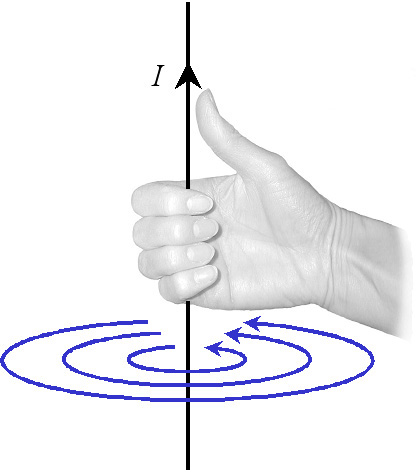
\includegraphics[width=0.4\linewidth]{Regla de la mano derecha.jpg}
    \caption{Regla de la mano derecha. Imágen obtenida de https://cluster-divulgacioncientifica.blogspot.com/2010/03/la-regla-de-la-mano-derecha.html}
\end{figure}

A partir de la ec 2. Podemos obtener el campo magnético que genera una espira cerrada.
\begin{equation*}
    \vec{B} = \frac{\mu _0 i}{2r} \hat{k}
\end{equation*}
Y si consideramos que es una bobina con n vuetlas, es decir, n espiras cerradas muy juntas, el campo magnético será:
\begin{equation}
    \vec{B} = \frac{\mu _0 i n}{2r} \hat{k}
\end{equation}

En el núcleo de la Tierra, hay metales magnéticos fundidos en movimiento, se estima que se mueven con una velocidad de al rededor de 40km por año, esto es suficiente para que se cree un campo magnético que es el causante de que las brújulas se orienten en un sentido. La magnitud de este campo magnético va a depender en dónde estemos situados, pero generalmente es de al rededor de 0.25-0.65 Gauss.
Los polos del campo magnético terrestre no se ubican exactamente en el polo geográfico de la tierra, de hecho están invertidos, es decir que el polo sur magnético  coincide con el polo norte geográfico, y el polo norte magnético con el polo sur geográfico, y difieren por un ángulo de 11.5°.
\begin{figure}[H]
    \centering
    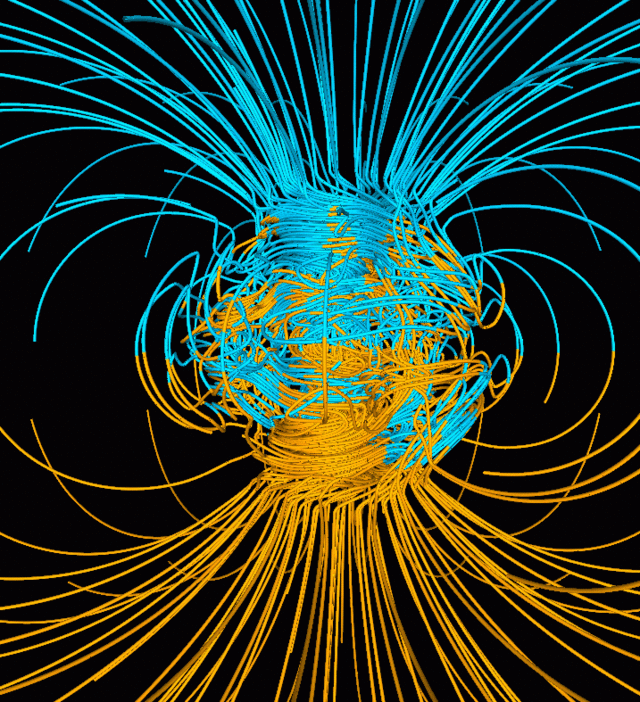
\includegraphics[width=0.5\linewidth]{tierra campo.png}
    \caption{Ilustración del campo magnético de la tierra}
\end{figure}
Un motor eléctrico convierte energía eléctrica en energía mecánica, mediante el uso de campos magnéticos. Un motor eléctrico muy simple consiste en un alambre deformado para que tenga dos "protuberancias", de tal manera que al acercarle un imán, una de las protuberancias quede más cerca del imán y la otra más alejada. Así, al pasar corriente por el alambre, va a experimentar la fuerza del campo magnético dada por la ec 1. de manera más intensa en la parte más cercana al imán. Y si le damos un eje de rotación adecuado, experimentará una torca, por lo que empezará a rotar y la parte del alambre que estaba más lejos, ahora quedara cercano al imán, dandole así un nuevo "impulso" para girar.


La temperatura de Curie es la temperatura en la que un material transiciona de una fase ferromagnética a una fase paramagnética, perdiendo así la propiedad de la magnetización. Usando esta idea es que se construye un péndulo de Curie. Que consiste en tener un material ferromagnético colgado como péndulo, adherido a un imán, y calentarlo hasta que llegue a la temperatura de Curie, para soltarse del imán y que al caer, pueda disminuir su temperatura recuperando las propiedades ferromagnéticas y adherirse al imán cuando regrese al punto inicial, para nuevamente calentarse y caer. Repitiendo la oscilación.
    \subsection{Hipótesis}
    Cuantitativamente, esperamos obtener un campo magnético terrestre de entre los 0.25-0.65 Gauss.

    Cualitativamente, esperamos que la limadura de hierro nos muestre un esbozo de las lineas de campo magnético que se generan; Además de una confirmación de la regla de la mano derecha con el orientamiento de las brújulas; También deberá girar el alambre en el arreglo del motor, siempre que tenga una corriente eléctrica fluyendo y el imán esté colocado correctamente; Y esperamos observar la pérdida de las propiedades ferromagnéticas del niquel al aumentar su temperatura y la recuperacion de estas propiedades al enfriarse.
    \subsection{Objetivos}
    \begin{itemize}
        \item Determinar el campo magnético de la tierra a partir del ángulo de deflección que provoca una bobina. 
        \item Visualizar las lineas de campo magnético.
        \item Verificar la regla de la mano derecha.
        \item Construir un motor eléctrico y un péndulo de Curie.
    \end{itemize} 
\section{Desarrollo Experimental / Métodos}
Este reporte consiste de varios experimentos, entonces será necesario identificar los materiales y procedimientos para cada uno por separado.
    \subsection{Campo magnético de la tierra}
        \subsubsection{Materiales}
        \begin{itemize}
            \item 1 Bobina de $\approx$30cm de diámetro 
            \item 1 Multímetro
            \item 1 Fuente de poder
            \item 2 Cables banana-banana
            \item 2 Caimanes
            \item 1 Flexómetro
            \item 3 Brújulas
            \item 2 Soportes universales
            \item 2 Nueces
            \item 2 Varillas
            \item Masking tape
            \item Pedazería de Cartón
        \end{itemize}
        Comenzamos montando la bobina de manera vertical. Con ayuda de los soportes universales, las nueces y las varillas, sostuvimos la bobina a una cierta altura (Nuestra bobina tenía unos orificios de plásico hechos para que pudieramos hacer uso de la varilla para montarla de esta forma). 
        
        Usando el flexómetro, medimos el diámetro de la bobina y determinamos su punto medio. Y a la altura del punto medio, se se colocó un pedazo de cartón para situar las 3 brújulas a esa altura.

        Ya colocadas las brújulas, se movió el arreglo de la bobina, de tal manera que estuviera alineado paralelamente con la brújula indicando al norte.
    
        Hecho esto, Conectámos la fuente de poder a la bobina fijando los cables con caimanes. La salida positiva en uno de los extremos de la bobina, y la negativa en el otro extremo.
        
        Ahora, dejámos únicamente la brújula que estaba en el centro para trabajar con ella, y el resto las retiramos. Finalmente fuimos poco a poco suministrando corriente eléctrica para desviar la brújula y registramos la corriente necesaria para que se desviara exactamente cada 5°, desde los 5° hasta los 45°.

        Es necesario saber tambíen el número de vuelas que tiene la bobina.
    \subsection{Líneas de campo magnético}
        \subsubsection{Materiales}
        \begin{itemize}
            \item 1 Hoja de papel
            \item Limadura de Hierro
            \item 1 Imán de Neodimio
            \item 1 Bobina
            \item 1 Fuente de poder
            \item 2 Cables banana-banana
            \item 2 Caimanes
            \item Lija de agua
        \end{itemize}
        Empezando por las líneas de campo del imán. Se colocó el imán recostado y la hoja de papel se sostuvo a una altura cercana al imán, Y se fue espolvoreando la limadura de hierro a la hoja desde arriba para que lograra adquirir la forma de las líneas.

        Ahora con la bobina, se conectó a la fuente de poder usando los cables banana-banana y los caimanes. Es necesario lijar las puntas en donde hace contacto con la fuente si tiene algún recubrimiento.
        Ya conectado, se le suministró un amperaje para generar el campo magnéticos, y ahora la hoja se colocó encima de la bobina. Y nuevamente se fue espolvoreando algo de limadura de hierro encima de la hoja.
    \subsection{Regla de la mano derecha}
        \subsubsection{Materiales}
        \begin{itemize}
            \item 1 Fuente de poder
            \item 2 Cables banana-banana
            \item 2 Caimanes
            \item 3 Brújulas
            \item Alambre de cóbre
            \item 2 Soportes universales
            \item 4 Nueces
            \item 4 Pinzas de 3 dedos
            \item 1 Lija de agua
            \item 1 Tabla agujerada de madera
        \end{itemize}
        Se montó un arreglo como el de la siguiente figura:
        \begin{figure}[H]
     \centering
    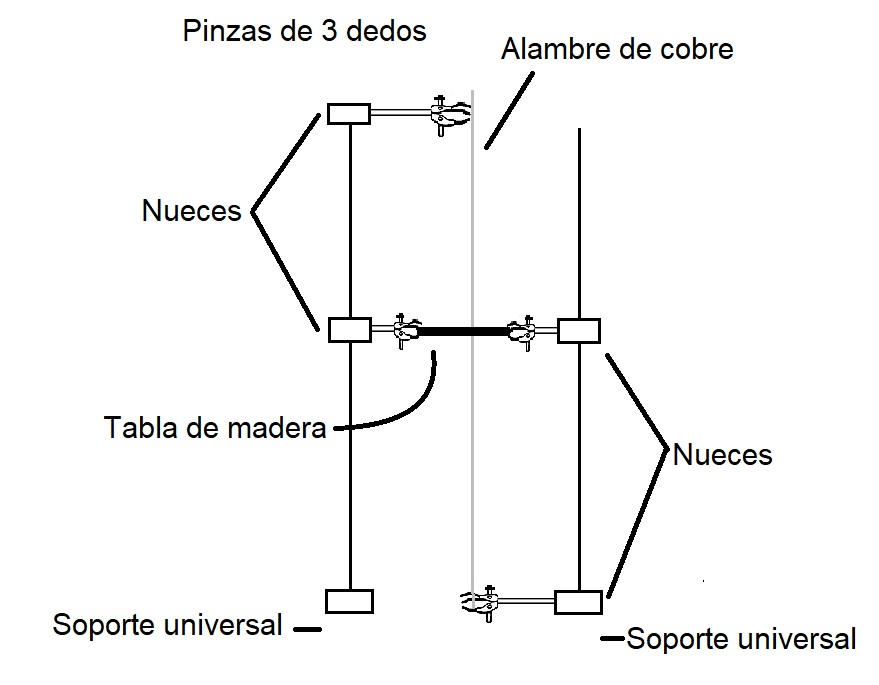
\includegraphics[width=0.75\linewidth]{Diagrama Mano derecha.jpg}
    \caption{Diagrama del experimento montado para la regla de la mano derecha}
    \end{figure}
    Se procuró que el alambre de cobre estuviera tenso para que fuera lo más recto posible. Luego colocamos las 3 brújulas en la tabla de madera, rodeando al alambre de cobre.
    Finalmente conectamos el alambre a la fuente de poder con los cables banana-banana y los caimanes. Nuevamente es necesario lijar las partes en donde hace contacto con la fuente si tiene algún recubrimiento.
    
    Se conectó el cable negativo a la parte positiva en el extremo superior del cable y el positivo en el extremo inferior y se suministró una corriente eléctrica.
    

    \subsection{Motor electromagnético}
        \subsubsection{Materiales}
        \begin{itemize}
            \item Alambre de cobre
            \item 1 Fuente de poder
            \item 2 Cables banana-banana
            \item 1 Lija de agua
            \item 2 Soportes universales
            \item 2 nueces
            \item 1 Imán de neodimio
            \item 1 Pinza de corte
        \end{itemize}
        Con el alambre de cobre se hizo una espira con dos extremos, dando varias vueltas y dos ganchos como se muestra en la imagen.
        \begin{figure}[H]
    \centering
    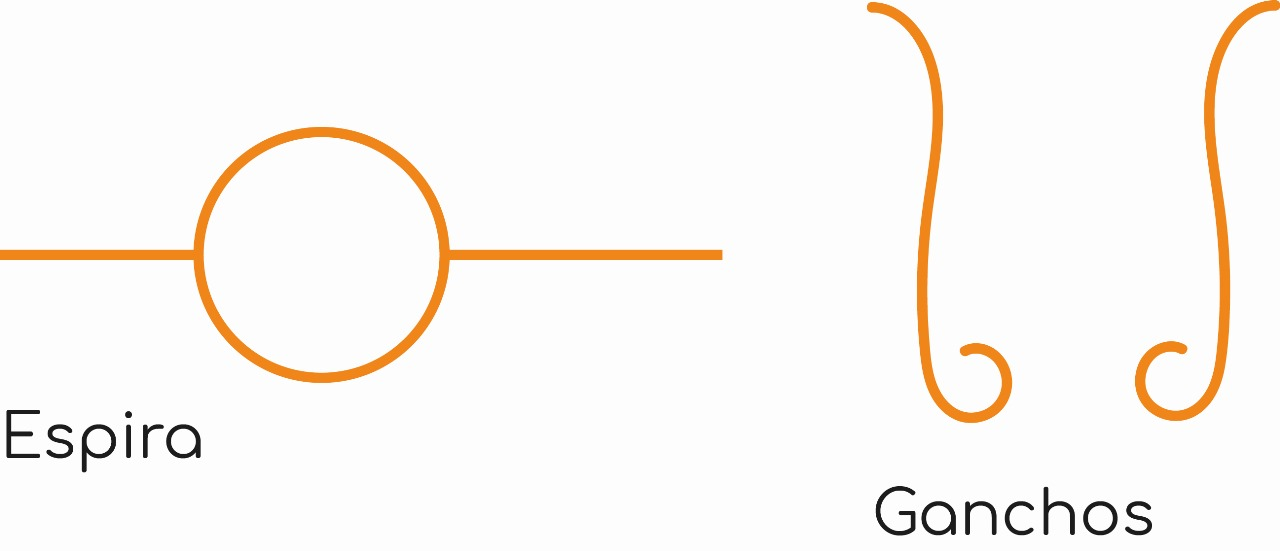
\includegraphics[width=0.6\linewidth]{DIagramaMotor1.jpg}
    \caption{Objetos hechos con el alambre de cobre}
        \end{figure}
        Después se hizo el siguiente arreglo con los ganchos y la espira.
        \begin{figure}[H]
    \centering
    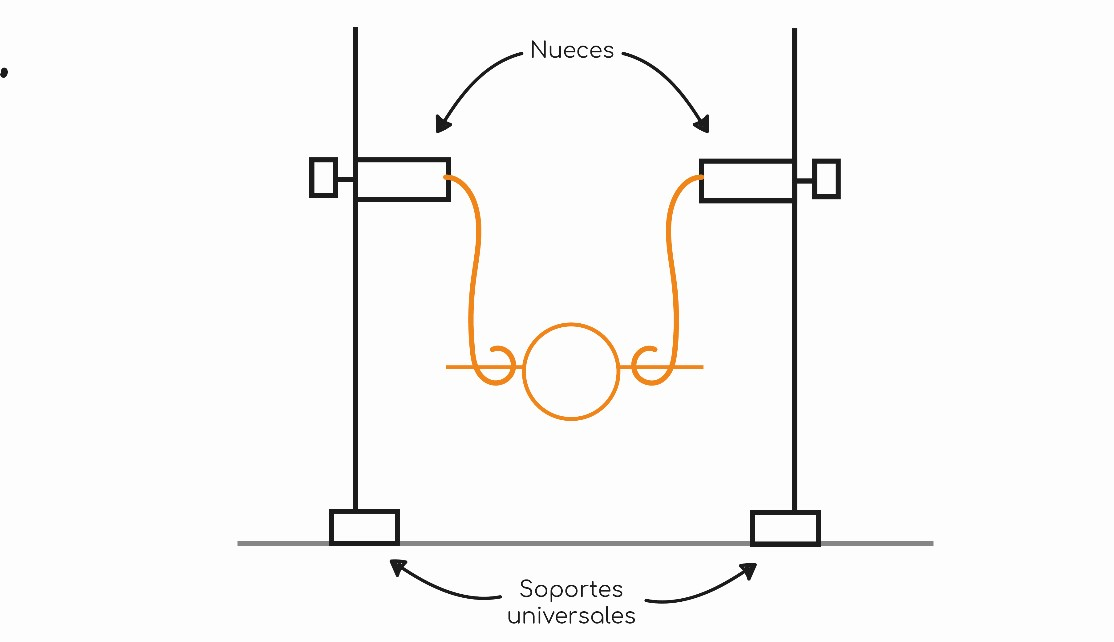
\includegraphics[width=0.85\linewidth]{DIagramaMotor2.jpg}
    \caption{Arreglo para el motor eléctrico}
        \end{figure}
        
        usando la nuez como soporte para el gancho, se conectaron los ganchos a la fuente de poder con los cables banana-banana y los caimanes.

        En cada parte del arreglo debe asegurarse que haya buen contacto, es decir, que esté bien lijado el alambre de cobre en las zonas de contacto.

        Una vez prendida la fuente, se le pasó una corriente eléctrica y se le acercó un imán de neodimio para que empezara a girar debido a la fuerza de Lorentz. El cómo acercar el imán depende de cómo esté inclinada la espira, entonces se debe procurar acercarlo a una de las concavidades del alambre que forma la espira.
    \subsection{Péndulo de Curie}
        \subsubsection{Materiales}
        \begin{itemize}
            \item 1 Moneda de níquel
            \item 1 Soporte universal
            \item 1 Vela
            \item 1 Imán de neodimio
            \item 1 Tornillo
            \item Hilo de cobre
            \item 1 Varilla
            \item 1 Nuez
        \end{itemize}
        Con los materiales se hizo el arreglo como se muestra a continuación:
        \begin{figure}[H]
    \centering
    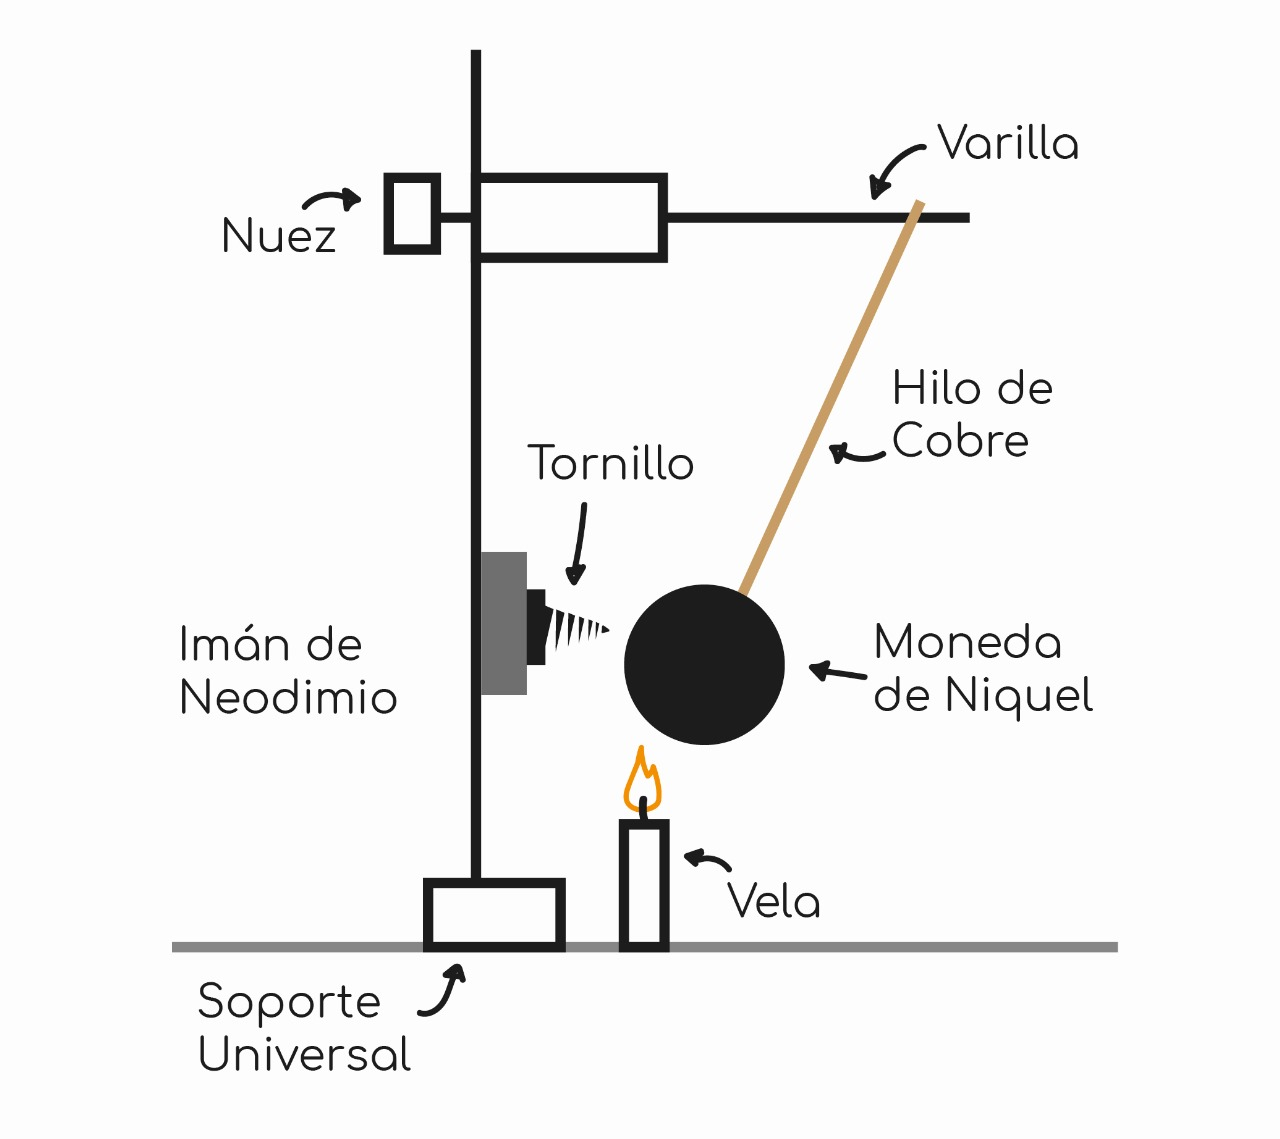
\includegraphics[width=0.6\linewidth]{DiagramaPendulo.jpg}
    \caption{Arreglo para un péndulo de Curie}
        \end{figure}
        Antes de encender la vela, la monedda de níquel debe estar inicialmente imantada al tornillo, y la lonigtud del hilo de cobre no debe ser pequeña (más de 30cm). Y ahora ya se debe encender la vela y esperar a que la moneda de níquel se caliente
        
\section{Resultados y discusión}
Para la primera parte \textbf{campo magnético de la tierra}, se ocupó una espira con radio de 0.304m y 94 vueltas, obtuvimos las siguientes tablas que relacionan ángulo de deflexión de la brújula al aumentar el amperaje, tangente de este ángulo y campo magnético en la espira.

\begin{table}[h]
\begin{tabular}{|c|c|c|c|}
\hline
Ángulo $\pm$ 2.5^{\circ} & Amperaje A $\pm$ 0.0005 & Tan angulo     & $B_b$            \\ \hline
0                                                                       & 0        & 0             & 0               \\ \hline
5                                                                       & 0.14     & 0.08748866353 & 0.000054399157  \\ \hline
10                                                                      & 0.293    & 0.1763269807  & 0.0001138496643 \\ \hline
15                                                                      & 0.566    & 0.2679491924  & 0.0002199280204 \\ \hline
20                                                                      & 0.749    & 0.3639702343  & 0.00029103549   \\ \hline
25                                                                      & 0.928    & 0.4663076582  & 0.0003605886978 \\ \hline
30                                                                      & 1.091    & 0.5773502692  & 0.0004239248592 \\ \hline
35                                                                      & 1.287    & 0.7002075382  & 0.000500083679  \\ \hline
40                                                                      & 1.548    & 0.8390996312  & 0.0006014992503 \\ \hline
45                                                                      & 2.01     & 1             & 0.0007810164684 \\ \hline
\end{tabular}
\caption{Primer registro de ángulo de deflexión, tangente del ángulo, amperaje y campo magnético de la espira.}
\end{table}

\begin{table}[h]
\begin{tabular}{|c|c|c|c|}
\hline
Ángulo $\pm$ 2.5^{\circ} & Amperaje A $\pm$ 0.0005 & Tan angulo     & $B_b$            \\ \hline
0                                                                       & 0        & 0.0000000000 & 0.0000000000 \\ \hline
5                                                                       & 0.159    & 0.0874886635 & 0.0000617819 \\ \hline
10                                                                      & 0.286    & 0.1763269807 & 0.0001111297 \\ \hline
15                                                                      & 0.425    & 0.2679491924 & 0.0001651403 \\ \hline
20                                                                      & 0.73     & 0.3639702343 & 0.0002836527 \\ \hline
25                                                                      & 0.812    & 0.4663076582 & 0.0003155151 \\ \hline
30                                                                      & 0.991    & 0.5773502692 & 0.0003850683 \\ \hline
35                                                                      & 1.113    & 0.7002075382 & 0.0004324733 \\ \hline
40                                                                      & 1.417    & 0.8390996312 & 0.0005505972 \\ \hline
45                                                                      & 1.749    & 1.0000000000 & 0.0006796009 \\ \hline
\end{tabular}
\caption{Segundo registro de ángulo de deflexión, tangente del ángulo, amperaje y campo magnético de la espira.}
\end{table}

\begin{table}[h]
\begin{tabular}{|c|c|c|c|}
\hline
Ángulo $\pm$ 2.5^{\circ} & Amperaje A $\pm$ 0.0005 & Tan angulo     & $B_b$            \\ \hline
0                                                                       & 0        & 0.0000000000 & 0.0000000000 \\ \hline
5                                                                       & 0.159    & 0.0874886635 & 0.0000596244 \\ \hline
10                                                                      & 0.286    & 0.1763269807 & 0.0001072490 \\ \hline
15                                                                      & 0.425    & 0.2679491924 & 0.0001593735 \\ \hline
20                                                                      & 0.73     & 0.3639702343 & 0.0002737474 \\ \hline
25                                                                      & 0.812    & 0.4663076582 & 0.0003044971 \\ \hline
30                                                                      & 0.991    & 0.5773502692 & 0.0003716215 \\ \hline
35                                                                      & 1.113    & 0.7002075382 & 0.0004173711 \\ \hline
40                                                                      & 1.417    & 0.8390996312 & 0.0005313700 \\ \hline
45                                                                      & 1.749    & 1.0000000000 & 0.0006558688 \\ \hline
\end{tabular}
\caption{Tercer registro de ángulo de deflexión, tangente del ángulo, amperaje y campo magnético de la espira.}
\end{table}

Al aplicar una regresión lineal entre el eje y definido por el campo magnético y el eje x definido por el inverso de la tangente de acuerdo a nuestros datos $0.553118G \pm 38.18\%$, estos datos en principio habían tenido valores absurdos y clase con clase los mejoramos, viendo que la fórmula que se propone con Biot-Savart era errada y se ocupaba en realidad una muy similar a la varilla infinita pero para el caso de la espira (que de hecho la deducción es muy distinta) es exactamente la misma pero sin un pi, además se debe ocupar la cotangente o en su defecto el inverso de la tangente, tal como hemos hecho. Según la literatura y lo reportado con el gaussometro los datos son coherentes pues deben ser muy similares a $0.3 \; gauss$ y en una región arbitraria de la tierra hasta $0.7 \; gauss$. \\

Para la parte de \textbf{líneas de campo magnético}, fue extremadamente complicado visualizar las líneas de campo magnéticos producidas por una espira a la que se le coloca corriente, pues incluso al llegar a la corriente máxima suministrada por la fuente de poder y con distintas espiras no se lograba apreciar. Para una espira en particular de número de vueltas no especificado al colocarla debajo de la hoja lo más pegado posible y colocar el amperaje máximo de la fuente (que incluso se sentía la corriente en el ambiente) logramos observar las siguientes líneas de campo. Nos parecen bastante acorde a lo que establece la teoría y de hecho se parece bastante al dibujo genérico que encuentra uno al buscar "líneas de campo" en google, i.e. el referente al dipolo magnético simple.


\begin{figure}[h]
    \centering
    
\includegraphics[width=0.5\linewidth]{image.png}
    \caption{Líneas de campo magnético generado por corriente en una espira}
    \label{fig:enter-label}
\end{figure}

En la misma parte se ocupó un imán de neodimio y con un arreglo análogo se consiguió ver lo siguiente.

\begin{figure}[h]
    \centering
    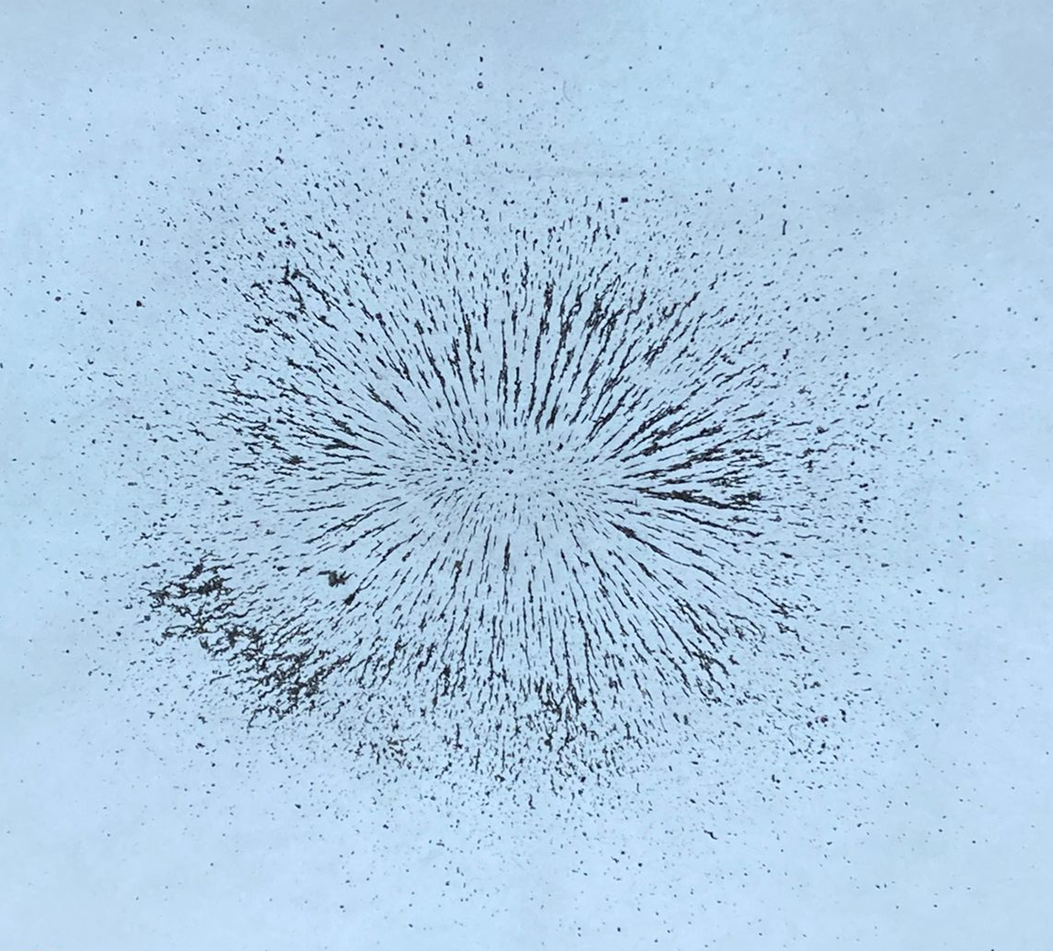
\includegraphics[width=0.5\linewidth]{iman.png}
    \caption{Líneas de campo producidas por imán permanente}
    \label{fig:enter-label}
\end{figure}

Que según la teoría es exactamente como debe verse.\\

Para la parte \textbf{regla de la mano derecha}, obtuvimos que las brújulas seguían un sentido antihorario cuando hacíamos pasar la corriente desde la parte baja positiva hasta la parte alta negativa, mientras que al intercambiar la posición de la corriente se invertía el sentido en el que giraban las brujulas, además al variar la cantidad de intensidad de corriente se deflectaban todavía más y seguían la misma trayectoria, tal como la regla de la mano derecha establece.

\begin{figure}[h]
    \centering
    \includegraphics[width=0.5\linewidth]{brujula.png}
    \caption{Arreglo para la demostración de la regla de la mano derecha}
    \label{fig:enter-label}
\end{figure}\\

Ahora, para la parte del \textbf{motor electromagnético}, lo esperado según la teoría es que debido al movimiento de las cargas que produce la corriente de la fuente de alto voltaje, cree un campo magnético, y que al interactuar con aquel del imán de neodimio para una trayectoria concreta del movimiento del imán se produzca un giro demasiado fuerte en la espira por la repulsión de los campos. Al inicio fue bastante complicado llegar al cortocircuito de la manera ideal pero eventualmente pudimos hacerlo girar durante un minuto.

\begin{figure}[h]
    \centering
    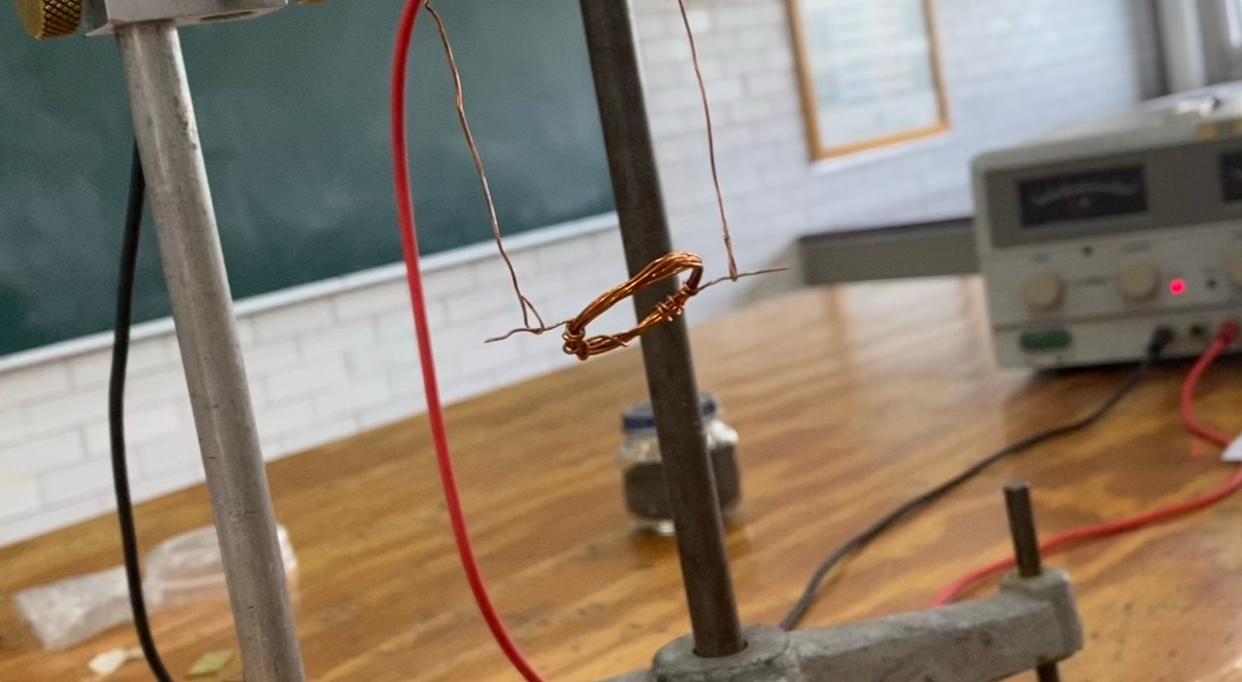
\includegraphics[width=0.6\linewidth]{espiracirculo.png}
    \caption{Arreglo del electroimán con una fuente de alto voltaje}
    \label{fig:enter-label}
\end{figure}

\newpage

Finalmente, para la parte del \textbf{péndulo de Curie}, teóricamente nos resultó imposible calcular posiciones en función de la masa, campo magnético transferido al tornillo del arreglo, etc. que nos ayudase, solo pudimos conocer que en al alcanzar la temperatura de Curie se pierden propiedades ferromagnéticas por lo que sugiere que para cierto tipo de arreglo va a oscilar entre una temperatura menor y mayor a este punto de quiebre por lo que adquirirá la forma de un péndulo; efectivamente pudimos ver que esto se logra después de un largo rato variando distancias, alturas y posiciones de la vela, largos del hielo entre otros parámetros.

\begin{figure}[h]
    \centering
    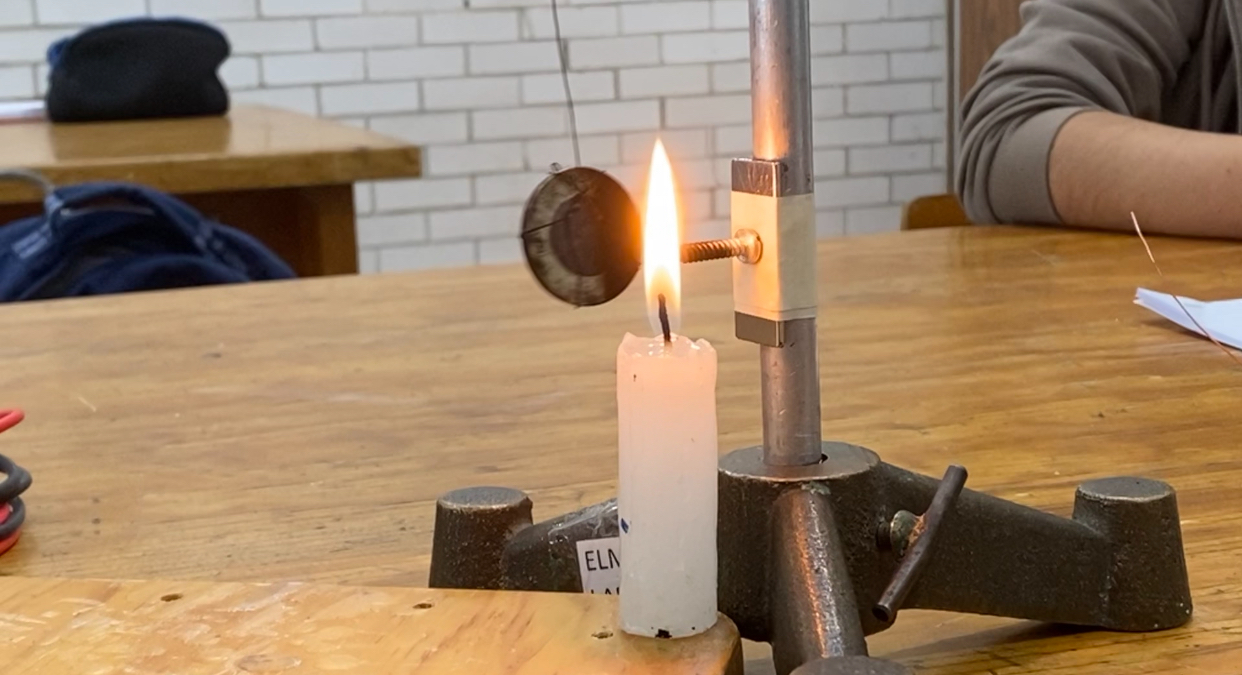
\includegraphics[width=0.75\linewidth]{pendulo curie.png}
    \caption{Péndulo de Curie}
    \label{fig:enter-label}
\end{figure}

\section{Conclusiones}

Esta investigación nos ha permitido explorar y verificar experimentalmente conceptos clave del electromagnetismo, iluminando teorías fundamentales y sus aplicaciones prácticas. Al replicar los hallazgos seminales de Ørsted, observamos directamente los efectos magnéticos producidos por corrientes eléctricas, ilustrando la profunda relación entre electricidad y magnetismo que se encuentra en el núcleo de la física moderna. Al medir el campo magnético terrestre, obtuvimos datos coherentes con los valores aceptados, validando así la fiabilidad de nuestras técnicas experimentales.

La visualización de las líneas de campo magnético mediante limaduras de hierro proporcionó representaciones concretas de los patrones de flujo magnético, alineándose estrechamente con las predicciones teóricas y enriqueciendo nuestra comprensión de las interacciones magnéticas. La aplicación de la regla de la mano derecha aclaró las características direccionales de los campos magnéticos alrededor de conductores, mientras que la construcción de un motor eléctrico simple demostró la transformación de la energía eléctrica en movimiento mecánico, destacando las aplicaciones prácticas de la fuerza de Lorentz; además, el experimento del péndulo de Curie nos permitió explorar la transición entre los estados ferromagnético y paramagnético, reforzando así el impacto de los cambios térmicos en las propiedades magnéticas. 


\newpage
\noindent {\bf Declaración de contribución de los autores}\\ 

Iván Bautista Alvarado$^1$ y Andrés López González$^1$ hemos realizado tanto el apartado escrito como el análisis de manera colectiva siendo una participación del 100\% por parte de ambos y no solo una repartición.\\ 

{\bf Agradecimientos} \\ 

A ese.\\

\begin{figure}[h]
    \centering
    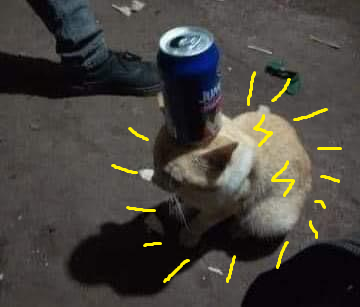
\includegraphics[width=0.5\linewidth]{el.png}
    \caption{Electrogato}
    \label{fig:enter-label}
\end{figure}\\

\begin{thebibliography}{99}

\bibitem{griffiths}
D. J. Griffiths, \textit{Introduction to Electrodynamics}, 3rd ed. Upper Saddle River, NJ, USA: Prentice-Hall, 1999.

\bibitem{jackson}
J. D. Jackson, \textit{Classical Electrodynamics}, 3rd ed. New York, NY, USA: Wiley, 1998.

\bibitem{sadiku}
M. N. O. Sadiku, \textit{Elements of Electromagnetics}, 6th ed. New York, NY, USA: Oxford University Press, 2014.

\bibitem{wangsness}
R. K. Wangsness, \textit{Electromagnetic Fields}, 2nd ed. New York, NY, USA: Wiley, 1986.

\bibitem{zangwill}
A. Zangwill, \textit{Modern Electrodynamics}. Cambridge, UK: Cambridge University Press, 2013.

\bibitem{purcell}
E. M. Purcell and D. J. Morin, \textit{Electricity and Magnetism}, 3rd ed. Cambridge, UK: Cambridge University Press, 2013.

\bibitem{shadowitz}
A. Shadowitz, \textit{The Electromagnetic Field}. Mineola, NY, USA: Dover Publications, 1988.


\end{thebibliography}


\end{document}